\documentclass[]{article}
% packages
%\usepackage[utf8]{vietnam}
\usepackage{amsmath, amssymb, amsthm}
\usepackage{color, graphicx, cases}
\usepackage{hyperref}
\hypersetup{
	colorlinks=true,
	linkcolor=black,
	filecolor=black,      
	urlcolor=black,
}
\usepackage{array, multirow, booktabs}
\usepackage{caption, subcaption}
\usepackage{ragged2e} % using justifying
\numberwithin{equation}{section}
\everymath{\displaystyle}
\usepackage{titling}

\usepackage[a4paper,left=35mm,top=31mm,right=20mm,bottom=30mm]{geometry}
\renewcommand{\baselinestretch}{1.5}

% new definitions
\newtheorem{dl}{Theorem}[section]
\newtheorem{md}{Proposition}[section]
\newtheorem{hq}{Corollary}[section]
\newtheorem{cy}{Remark}[section]

\theoremstyle{definition}
\newtheorem{dn}{Definition}[section]
\newtheorem{vd}{Example}[section]
\newtheorem{bt}{Problem}[section]
\newtheorem{nx}{Comment}[section]

% reference
\usepackage{cleveref}
\crefname{dl}{\textbf{Theorem}}{}
\crefname{md}{\textbf{Proposition}}{}
\crefname{hq}{\textbf{Corollary}}{}

\crefname{dn}{\textbf{Definition}}{}
\crefname{vd}{\textbf{Example}}{}
\crefname{cy}{\textbf{Remark}}{}
\crefname{bt}{\textbf{Problems}}{}
\crefname{nx}{\textbf{Comment}}{}
\everymath{\displaystyle}
\begin{document}
\justifying

\thispagestyle{empty}

\newpage
\section{Introduction}
Consider a physical domain $\Omega \subset \mathbb{R}^d,\, d\in \mathbb{N^+}$ be bounded with the boundary $\Gamma$ and donate $Q:=\Omega\times (0,\, T)$ and $ S:=\Gamma \times (0,\, T)$ with $T>0$ given. 
\\
Consider the heat equation
\begin{align}\label{1.1}
	\frac{\partial u}{\partial t}-\sum_{i, j=1}^{d}\frac{\partial}{\partial x_j}\left(a_{ji}(x, t)\frac{\partial u}{\partial x_i}\right)=F(x, t), \quad(x, t)\in Q,
\end{align}
with the initial and Dirichlet conditions, respectively
\begin{align}
	u(x, 0)&=u_0(x),\quad x\in \Omega,\label{1.2}\\
	u(x, t)&=\varphi(x, t),\quad(x, t)\in S \label{1.3}
\end{align}
where
\begin{align*}
	&a_{ij}\in L^{\infty}(Q),\, a_{ij}=a_{ji},\; \forall i, j\in \{1, 2, ..., d\},\\
	&\lambda_1\left\|\xi\right\|^2\leq \sum_{i, j=1}^{d}a_{ij}\xi_i\xi_j\leq \lambda_2\left\|\xi\right\|^2,\; \forall \xi\in\mathbb{R}^d,\\
	&\varphi\in L^2(S),\; u_0\in L^2(\Omega),\; F\in L^2(0,\, T;\, H^{-1}(\Omega)),
\end{align*}
with $\lambda_1$ và $\lambda_2$ are positive constants.
\\
The direct problem is to determine $u$ when all data $a_{ji}, i, j=\overline{1, d}, \,u_0, \,\varphi$ and $F$ in \cref{1.1,1.2,1.3} are given. On the other hand, the inverse problem (IP) is to identify a missed data such as the right hand side $F$ when some additional observation on the solution $u$ are available. 
\\
Consider the right hand side of equation \eqref{1.1} following the form $F(x, t)=f(.)q(x, t)+g(x, t)$, with $q,\, g$ are given and $f(.)$ is either $f(x, t)$, $f(x)$ or $f(t)$. Denote $N_m$ is the number of measurements and $\ell_k u(f) =\omega_k, k=\overline{1, N_m}$ is the value of the $kth$ measurement. We have different inverse problems depending on either the form of $F$ or the observation on the solution $u$: 
\begin{itemize}
	\item IP1: Find $f(.)$ if $u(x, t)$ is given on $Q$. So that $N_m=1$ and $\ell_ku(x, t)=u(x, t)=\omega_k(x, t), \; (x, t)\in Q,\, k=\overline{1, N_m}$.
	\item IP2: Find $f(.)$ if $\ell_ku=\int_\Omega w_k(x)u(x, t)dx=\omega_k(t)$ and $w_k(x)>0, \forall x\in \Omega$ are given. This observation called \textit{integral observation}. Furthermore, an observation derives from integral observation called \textit{point observation} if $w_k(x)$ is a dirac delta function $\delta_k(x-x_k)$, so that $\ell_k(t)=\int_\Omega\delta_k(x-x_k)u(x, t)dx=u(x_k, t)=\omega_k(t)$.
\end{itemize}
To solve this problem, we need to minimize the least square functional 
$$J_{\gamma}(f)=\frac{1}{2}\sum_{k=1}^{N_{o}}\left\|\ell_k u(f)-\omega_k\right\|_{L^2(*)}^2.$$
However, this minimization problem is unstable and there might be many minimizers to it. Therefore, we minimize the Tikhonov functional instead
$$J_{\gamma}(f)=\frac{1}{2}\sum_{k=1}^{N_{o}}\left\|\ell_k u(f)-\omega_k\right\|_{L^2(*)}^2+\frac{\gamma}{2}\left\|f-f^*\right\|_{L^2(**)}^2,$$
with $\gamma>0$ being a regularization parameter, $f^*$ is an a prior estimation of $f$ and $\left\|.\right\|_{L^2(*)}$ and $\left\|.\right\|_{L^2(**)}$ respectively depends on $w_k(*)$ and $f(**)$ appropriately.

\section{Variational problem}
To introduce the concept of weak form, we use the standard Sobolev spaces $H^1(\Omega),\, H^1_0(\Omega),\, H^{1, 0}(Q)$ and $H^{1, 1}(Q)$. Further, for a Banach space $B$, we define
$$L^2(0, T; B)=\left\{u:u(t)\in B \text{ a.e } t\in (0, T) \text{ and } \left\|u\right\|_{L^2(0, T; B)} <\infty \right\},$$
with the norm
$$\left\|u\right\|_{L^2(0, T; B)}=\int_0^T\left\|u(t)\right\|^2_Bdt.$$
In the sequel, we shall use the space $W(0, T)$ define as
$$W(0, T)=\left\{u: u\in L^2(0, T; H^1(\Omega)), u_t\in L^2\left(0, T; \left(H^1(\Omega)\right)'\right) \right\}$$
Suppose that $F\in L^2(Q)$, a week solution in $W(0, T)$ of the problem \cref{1.1,1.2,1.3} is a function $u(x, t)\in W(0, T)$ satisfying the identity
\begin{align}\label{2.1}
	\int_{Q}\left[\frac{\partial u}{\partial t}v+\sum_{i, j=1}^{d}a_{ji}\frac{\partial u}{\partial x_i}\frac{\partial v}{\partial x_j}\right]dxdt=\int_{Q}Fvdxdt,\;\forall v \in L^2\left(0, T; H^1(\Omega)\right).
\end{align}
and 
\begin{align}\label{2.2}
	u(x, 0)=u_0,\; x\in \Omega.
\end{align}
\begin{align}\label{2.3}
	\left\|u\right\|_{L^2(0, T; B)} \leq c_d \left(\left\|F\right\|_{L^2(Q)}+\left\|u_0\right\|_{L^2(\Omega)}+\left\|\varphi\right\|_{L^2(S)}\right)
\end{align}
We suppose that $F$ has the form $F(x, t)=f(x, t)q(x, t)+g(x, t)$ with $f\in L^2(Q),\, q\in L^\infty(Q)$ and $g\in L^2(Q)$. We hope to recover $f(x, t)$ from the observation. Since the solution $u(x, t)$ depends on the function $f(x, t)$, so we denote it by $u(x, t, f)$ or $u(f)$. Identify $f(x, t)$ satisfying 
$$\ell_k u(f)=\omega_k,\; \forall k = \overline{1, N_o}$$
where $\ell_k u(f)$ is the observation on the solution depending on $f$. We suppose to solve (IP2) problem and (IP1) will be done the same way. We need to minimize the Tikhonov functional
\begin{align}\label{2.4}
	J_{\gamma}(f)=\frac{1}{2}\sum_{k=1}^{N_m}\left\|\ell_k u(f)-\omega_k\right\|_{L^2(0, T)}^2+\frac{\gamma}{2}\left\|f-f^*\right\|_{L^2(Q)}^2.
\end{align}

We will prove that $J_\gamma$ is Frechet differentiable and drive a formula for its gradient. In doing so, we need the adjoint problem
\begin{align}\label{2.5} 
	\begin{cases}
		-\frac{\partial p}{\partial t}-\sum_{i, j=1}^{d}\frac{\partial}{\partial x_j}\left(a_{ji}(x, t)\frac{\partial p}{\partial x_i}\right)=\sum_{k=1}^{N_m}w(x)\left(\ell_k u(f)-\omega_k\right), & (x, t)\in Q,\\
		u(x, t)=0, & (x, t)\in S\\
		p(x, T)=0, & x\in \Omega.
	\end{cases}
\end{align}
By changing the time direction, meaning $\overline{p}(x, t)=p(x, T-t)$, we will get a Dirichlet problem for parabolic equations.
\begin{dl}
	The functional $J_\gamma$ is Frechet differentiable and its gradient $\nabla J_\gamma$ at $f$ has the form 
	\begin{align}\label{2.6}
		\nabla J_\gamma(f)=q(x, t)p(x, t)+\gamma \left(f(x, t)-f^*(x, t)\right)
	\end{align}
\end{dl}
\begin{proof}
	By taking a small variation $\delta f \in L^2(Q)$ of $f$ and denoting $\delta u(f)=u(f+\delta f)-u(f)$, we have
	\begin{align*}
		J_0(f+\delta f)-J_0(f)&=\frac{1}{2}\sum_{k=1}^{N_m}\left\|\ell_k u(f+\delta f)-\omega_k\right\|^2_{L^2(0, T)}-\frac{1}{2}\sum_{k=1}^{N_m}\left\|\ell_k u(f)-\omega_k\right\|^2_{L^2(0, T)}\\
		&=\frac{1}{2}\sum_{k=1}^{N_m}\left\|\ell_k \delta u(f) +\ell_k u(f)-\omega_k\right\|^2_{L^2(0, T)}-\frac{1}{2}\sum_{k=1}^{N_m}\left\|\ell_k u(f)-\omega_k\right\|^2_{L^2(0, T)}\\
		&=\sum_{k=1}^{N_m}\frac{1}{2}\left\|\ell_k \delta u(f)\right\|^2_{L^2(0, T)}+\sum_{k=1}^{N_m}\left\langle \ell_k \delta u(f), \ell_k u(f)-\omega_k\right\rangle_{L^2(0, T)},
	\end{align*}
	where $\delta u(f)$ is the solution to this problem
	\begin{align}\label{2.7}
		\begin{cases}
			\frac{\partial \delta u}{\partial t}-\sum\limits_{i, j=1}^{d}\frac{\partial}{\partial x_j}\left(a_{ji}(x, t)\frac{\partial \delta u}{\partial x_i}\right)=q(x, t)\delta f,&(x, t)\in Q,\\
			\delta u(x, t)=0, & (x, t)\in S,\\
			\delta u(x, 0)=0, &x\in \Omega.
		\end{cases}
	\end{align}
	Because the priori estimate \eqref{2.3} for the direct problem, we have
	\begin{align*}
		\left\|\ell_k\delta u(f)\right\|_{L^2(0, T)}^2=o\left(\left\|\delta f\right\|_{L^2(Q)}\right)\, \text{when } \left\|\delta f\right\|_{L^2(Q)}\to 0.
	\end{align*}
	What is more, applying the Green formula for \eqref{2.5} and \eqref{2.7}, we get
	$$\sum_{k=1}^{N_m}\int_{Q} \delta u(x, t) w(x) \left(\ell_k u(f)-\omega_k(t)\right)dxdt=\int_{Q} p(x, t)q(x, t)\delta f(x, t)dxdt$$
	Therefore,
	\begin{align*}
		J_0(f+\delta f)-J_0(f)&=\sum_{k=1}^{N_m}\int_{Q}\delta u(x, t)w(x)\left(\ell_k u(f)-\omega_k(t)\right)ds+o\left(\left\|\delta f\right\|_{L^2(Q)}\right)\notag\\
		&=\int_Q q(x, t)p(x, t)\delta f(x, t)dxdt+o\left(\left\|\delta f\right\|_{L^2(I)}\right)\notag\\
		&=\left\langle qp,\delta f \right\rangle_{L^2(Q)}+o\left(\left\|\delta f\right\|^2_{L(Q)}\right).
	\end{align*}
	Therefore, we will obtain
	$$J_\gamma(f+\delta f)-J_\gamma(f)=\left\langle qp,\delta f \right\rangle_{L^2(Q)}+\gamma\left\langle f-f^*,\delta f \right\rangle_{L^2(Q)}+o\left(\left\|\delta f\right\|^2_{L(Q)}\right).$$
	Hence the functional $J_\gamma$ is Frechet differentiable and its gradient $\nabla J_\gamma$ at $f$ has the form \eqref{2.5}. The theorem is proved.
\end{proof}
\begin{cy}
	In this theorem, we write the Tikhonov functional for $F(x, t)=f(x, t)q(x, t)+g(x, t)$. But when F has another form, the penalty term should be modified
	\begin{itemize}
		\item $F(x, t)=f(x)q(x, t)+g(x, t)$: the penalty functional is $\left\|f-f^*\right\|_{L^2(\Omega)}$ and $$\nabla J_0(f)=\int_0^Tq(x, t)p(x, t)dt.$$
		\item $F(x, t)=f(t)q(x, t)+g(x, t)$: the penalty functional is $\left\|f-f^*\right\|_{L^2(0, T)}$ and $$\nabla J_0(f)=\int_\Omega q(x, t)p(x, t)dt.$$
	\end{itemize}
\end{cy}
\noindent To find $f$ satisfied \eqref{2.4}, we use the conjugate gradient method (CG). Its iteration follows, we assume that at the $k$th iteration, we have $f^k$ and then the next iteration will be
$$f^{k+1}=f^k+\alpha_kd^k,$$
with
\begin{align*}
	d^k&=\left\{\begin{array}{ll}
	-\nabla J_\gamma(f^k),& k=0,\\
	-\nabla J_\gamma(f^k)+\beta_kd^{k-1},& k>0,
	\end{array}\right.\\\\
	\beta_k&=\frac{\left\|\nabla J_\gamma (f^k)\right\|^2_{L^2(I)}}{\left\|\nabla J_\gamma (f^{k-1})\right\|^2_{L^2(I)}},
\end{align*}
and
$$\alpha_k=\operatorname*{arg\,min}_{\alpha\geq 0}J_\gamma(f^k+\alpha d^k).$$
To identify $\alpha_k$, we consider two problems
\begin{bt}\label{bt2.1}
	Denote the solution of this problem is $u[f]$
	\begin{align*}
		\begin{cases}
			\frac{\partial u}{\partial t}-\sum_{i, j=1}^{d}\frac{\partial}{\partial x_j}\left(a_{ji}(x, t)\frac{\partial u}{\partial x_i}\right)=f(x, t)h(x, t),&(x, t)\in Q,\\
			u(x, t)=0, & (x, t)\in S,\\
			u(x, 0)=0,&x\in \Omega.
		\end{cases}
	\end{align*}
\end{bt}
\begin{bt}\label{bt2.2}
	Denote the solution of this problem is $u(u_0, \varphi)$
	\begin{align*}
		\begin{cases}
			\frac{\partial u}{\partial t}-\sum_{i, j=1}^{d}\frac{\partial}{\partial x_j}\left(a_{ji}(x, t)\frac{\partial u}{\partial x_i}\right)=g(x, t),&(x, t)\in Q,\\
			u(x, t)=\varphi(x, t), & (x, t)\in S,\\
			u(x, 0)=u_0(x),&x\in \Omega.
		\end{cases}
	\end{align*}
\end{bt}
\noindent If so, the observation operators have the form $\ell_i u(f)=\ell_i u[f]+\ell_i u(u_0, \varphi)=A_if+\ell_i u(u_0, \varphi)$, with $A_i$ being bounded linear operators from $L^2(Q)$ to $L^2(0, T)$.\\
We have
\begin{align*}
	J_{\gamma}(f^k+\alpha d^k)&=\frac{1}{2}\sum_{i=1}^{N_m}\left\|\ell_i u(f^k+\alpha d^k)-\omega_i\right\|_{L^2(0, T)}^2+\frac{\gamma}{2}\left\|f^k+\alpha d^k-f^*\right\|_{L^2(Q)}^2\\[0.2cm]
	&=\frac{1}{2}\sum_{i=1}^{N_m}\left\|\alpha A_id^k+A_if^k+\ell_i u(u_0, \varphi)-\omega_i\right\|_{L^2(0, T)}^2+\frac{\gamma}{2}\left\|f^k+\alpha d^k-f^*\right\|_{L^2(Q)}^2\\[0.2cm]
	&=\frac{1}{2}\sum_{i=1}^{N_m}\left\|\alpha A_id^k+\ell_i u(f^k)-\omega_i\right\|_{L^2(0, T)}^2+\frac{\gamma}{2}\left\|f^k+\alpha d^k-f^*\right\|_{L^2(Q)}^2.
\end{align*}
Differentiating $J_\gamma(f^k+\alpha d^k)$ with respect to $\alpha$, we get
\begin{align*}
	\frac{\partial J_\gamma(f^k+\alpha d^k)}{\partial \alpha} &= \alpha\sum_{i=1}^{N_m}\left\|A_id^k \right\|_{L^2(0, T)}^2+\sum_{i=1}^{N_m}\left\langle A_id^k,\ell_i u(f^k)-\omega_i\right\rangle_{L^2(0, T)}\\[0.2cm]
	&\quad+\gamma\alpha\left\| d^k\right\|_{L^2(Q)}^2+\gamma\left\langle d^k, f^k-f^*\right\rangle_{L^2(Q)}.
\end{align*}
Putting $\frac{\partial J_\gamma(f^k+\alpha d^k)}{\partial \alpha}=0$, we obtain
\begin{align*}
	\alpha_k&=-\frac{\sum_{i=1}^{N_m}\left\langle A_id^k, \ell_i u(f^k)-\omega_i\right\rangle_{L^2(0, T)}+\gamma\left\langle d^k, f^k-f^*\right\rangle_{L^2(Q)}}{\sum_{i=1}^{N_m}\left\|A_id^k\right\|^2_{L^2(0, T)}+\gamma\left\|d^k\right\|^2_{L^2(Q)}}\\[0.2cm]
	&=-\frac{\sum_{i=1}^{N_m}\left\langle d^k, A_i^*\left(\ell_i u(f^k)-\omega_i\right)\right\rangle_{L^2(Q)}+\gamma\left\langle d^k, f^k-f^*\right\rangle_{L^2(Q)}}{\sum_{i=1}^{N_m}\left\|A_id^k\right\|^2_{L^2(0, T)}+\gamma\left\|d^k\right\|^2_{L^2(Q)}}\\[0.2cm]
	&=-\frac{\sum_{i=1}^{N_m}\left\langle d^k, A_i^*\left(\ell_i u(f^k)-\omega_i\right)+\gamma(f^k-f^*)\right\rangle_{L^2(Q)}}{\sum_{i=1}^{N_m}\left\|A_id^k\right\|^2_{L^2(0, T)}+\gamma\left\|d^k\right\|^2_{L^2(Q)}}\\[0.2cm]
	&=-\frac{\left\langle d^k,\nabla J_\gamma(f^k)\right\rangle_{L^2(Q)}}{\sum_{i=1}^{N_m}\left\|A_id^k\right\|^2_{L^2(0, T)}+\gamma\left\|d^k\right\|^2_{L^2(Q)}}.
\end{align*}
Because of $d^k=r^k+\beta_kd^{k-1},\, r^k=-\nabla J_\gamma (f^k)$ and $\left\langle r^k,d^{k-1}\right\rangle_{L^2(I)}=0$, we get 
$$\alpha_k=\frac{\left\|r^k\right\|^2_{L^2(Q)}}{\sum_{i=1}^{N_m}\left\|A_id^k\right\|^2_{L^2(0, T)}+\gamma\left\|d^k\right\|^2_{L^2(Q)}}.$$

\noindent \textbf{CG algorithm}
\begin{itemize}
	\item[1.] Set $k=0$, initiate $f^0$.
	\item[2.] For $k=0, 1, 2,...$. Calculate
	$$r^k=-\nabla J_\gamma(f^k).$$
	Update\\
	\begin{align*}
		d^k&=\left\{\begin{array}{ll}
		r^k,& k=0,\\
		r^k+\beta_kd^{k-1},& k>0,
		\end{array}\right.\\\\
		\beta_k&=\frac{\left\|r^k\right\|^2_{L^2(Q)}}{\left\|r^{k-1}\right\|^2_{L^2(Q)}}.
	\end{align*}
	\item[3.] Calculate
	$$\alpha_k=\frac{\left\|r^k\right\|^2_{L^2(Q)}}{\sum_{i=1}^{N_m}\left\|A_id^k\right\|^2_{L^2(0, T)}+\gamma\left\|d^k\right\|^2_{L^2(Q)}}.$$
	Update
	$$f^{k+1}=f^{k}+\alpha_kd^k.$$
\end{itemize}

\section{Finite element method}
We rewrite the Tikhonov functional
\begin{align*}
	J_\gamma(f)&=\frac{1}{2}\sum_{i=1}^{N_m}\left\|\ell_i u[f]+\ell_i u(u_0, \varphi)-\omega_i\right\|^2_{L^2(0, T)}+\frac{\gamma}{2}\left\|f-f^*\right\|^2_{L^2(Q)}\\
	&=\frac{1}{2}\sum_{i=1}^{N_m}\left\|A_if+\ell_i u(u_0, \varphi)-\omega_i\right\|^2_{L^2(0, T)}+\frac{\gamma}{2}\left\|f-f^*\right\|^2_{L^2(Q)}\\
	&=\frac{1}{2}\sum_{i=1}^{N_m}\left\|A_if-\hat{\omega}_i\right\|^2_{L^2(0, T)}+\frac{\gamma}{2}\left\|f-f^*\right\|^2_{L^2(Q)},
\end{align*}
with $\hat{\omega}_i=\omega_i-\ell_i u(u_0, \varphi)$.
\\
The solution $f^\gamma$ of the minimization problem \eqref{2.4} is characterized by the first-order optimality condition
\begin{align}\label{3.1}
	\nabla J_\gamma(f^\gamma)= \sum_{i=1}^{N_m}A^*_i(A_if^\gamma-\hat{\omega}_i)+\gamma(f^\gamma-f^*)=0,
\end{align}
with $A_i^*: L^2(0, T)\to L^2(Q)$ is the adjoint operator of $A_i$ defined by $\sum_{i=1}^{N_m}A_i^*\left(\ell_i u(f) - \omega_i\right) = p$ where $p$ is the solution of the adjoint problem \eqref{2.5}. 

\subsection{Finite element approximate of $A_k,\, A_k^*$}
We will approximate \eqref{3.1} by using the space-time finite element method with finite spaces $X_h \subset Y_h$. For the space-time domain $Q=\Omega\times I\subset \mathbb{R}^{d+1}$, we consider a sequence of admissible decompositions $Q_h$ into shape regular simplicity finite element $q_l$
$$Q_h=\cup_{l=1}^{N}\bar{q}_l.$$
Denote $\left\lbrace (x_k, t_k)\right\rbrace_{k=1}^M $ is a set of nodes $(x_k, t_k)\in \mathbb{R}^{d+1}$. We introduce a reference element $q\in \mathbb{R}^{d+1}$ which any element $q_l$ can maple to $q$ by using
$$\begin{pmatrix}x\\t\end{pmatrix}=\begin{pmatrix}x_k\\t_k\end{pmatrix}+J_l\begin{pmatrix}\xi\\\tau\end{pmatrix}, \; \begin{pmatrix}\xi\\\tau\end{pmatrix}\in q.$$
with $\Delta_l$ is the volume of $q_l$ 
$$\Delta_l=\int_{q_l}dxdt=\det J_l\int_q d\xi d\tau=|q|\det J_l,$$
and the local mesh width
$$h_l=\Delta_l^{\frac{1}{d+1}},\; h:=\max_{l=1, ..., N}h_l.$$
Note that
$$|q|=\begin{cases}
	\frac{1}{2},& d=1,\\[0.1cm]
	\frac{1}{6},& d=2.
\end{cases}$$
%phương trình biến phân xấp xỉ
\begin{align}\label{3.2}
	\int_{Q}\left[\frac{\partial u_h}{\partial t}v_h+\sum_{i, j=1}^{d}a_{ji}\frac{\partial u_h}{\partial x_i}\frac{\partial v_h}{\partial x_j}\right]dxdt=\int_{Q}Fv_hdxdt+\int_{S}\varphi v_hdsdt, \forall v_h\in Y_h.
\end{align}
and 
\begin{align}\label{3.3}
	u_h(x, 0)=u_0, x\in \Omega.
\end{align}
\\
The discrete variational problem \eqref{3.2} admits a unique solution $u_h\in X_h$. Hence, the discrete version of the optimal control problem will be
$$J_{\gamma, h}(f)=\frac{1}{2}\sum_{i=1}^{N_m}\left\|A_{i, h}f-\hat{\omega}_{i, h}\right\|^2_{L^2(0, T)}+\frac{\gamma}{2}\left\|f-f^*\right\|^2_{L^2(Q)}.$$
Let $f^\gamma_h$ be the solution of this problem is characterized by the variational equation
\begin{align}\label{3.4}
	\nabla J_{\gamma, h}(f^\gamma_h)= \sum_{i=1}^{N_m}A_{i, h}^*(A_{i, h}f^\gamma-\hat{\omega}_{i, h})+\gamma(f^\gamma_h-f^*)=0,
\end{align}
where $A_{i, h}^*$ is the adjoint operator of $A_{i, h}$. But it is hardly to find $A^*_{i, h}$ from $A_{i, h}$ in practice. So we define a proximate $\hat{A}_{i, h}^*$ of $A_i^*$ instead. In deed, we have $\sum_{i=1}^{N_m}\hat{A}^*_{i, h}\left(\ell_i u(f) - \omega_i\right)=p_h$, with $p_h$ is the approximate solution of adjoint problem \eqref{2.5}. Therefore, the equation above will be
\begin{align}\label{3.5}
	\nabla J_{\gamma, h}(f^\gamma_h)\simeq\nabla J_{\gamma, h}(\hat{f}^\gamma_h)= \sum_{i=1}^{N_m}\hat{A}_{i, h}^*(A_{i, h}\hat{f}^\gamma-\hat{\omega}_{i, h})+\gamma(\hat{f}^\gamma_h-f^*)=0,
\end{align}
Moreover, the observation will have noise in pratice, so instead of $\omega(x, t)$, we only get $\omega^{\delta}(x, t)$ satisfy
$$\left\| \omega-\omega^\delta\right\|_{L^2(S_1)}\leq \delta.$$
Therefore, instead of getting $\hat{f}^\gamma_h$ satisfies the equation \eqref{3.5}, we will get $\hat{f}^{\gamma, \delta}_h$ satisfies
\begin{align}\label{3.6}
	\nabla J_{\gamma, h}\left(\hat{f}^{\gamma, \delta}_h\right)= \sum_{i=1}^{N_m}\hat{A}_{i, h}^*(A_{i, h}\hat{f}^{\gamma, \delta}_h-\hat{\omega}_{i, h}^\delta)+\gamma(\hat{f}^{\gamma, \delta}_h-f^*)=0,
\end{align}
with $\hat{\omega}_{i, h}^\delta=\omega^\delta-\ell_i u_h(u_0, \varphi)$.
\subsection{Convergence results}
\begin{dl}\label{dl3.2}
	Let $u(x, t)$ be the solution of variational problem \eqref{2.1} - \eqref{2.2} and $u_h(x, t)$ be the solution for \eqref{3.2} - \eqref{3.3} Then there holds the error estimate
	\begin{align}\label{3.7}
		\left\| u-u_h\right\|_{L^2(Q)}\leq \left\| u-u_h\right\|_{L^2(I;\; H^1(\Omega))}\leq c_2h_{xt} \left|u\right|_{H^2(\Omega)}.
	\end{align}
\end{dl}
\noindent What is more,
\begin{align*}
	\left\| \left(A^*-\hat{A}^*_h\right)\phi\right\|_{L^2(Q)}^2=\int_Q (p-p_h)^2dxdt=\left\| p-p_h\right\|_{L^2(Q)}^2
\end{align*}
\begin{align}\label{3.8}
	\Rightarrow \left\| \left(A^*-A^*_h\right)q\right\|_{L^2(I)}\leq c_5h.
\end{align}
Let $u_h[f]$ và $u_h(u_0, \varphi)$ are the approximate solutions of \cref{bt2.1} and \cref{bt2.2} by using space-time finite element method. We define $A_h$ of $A$ is $A_hf=\ell u_h[f]$ and $\hat{\omega}_h=\omega-\ell u_h(u_0, \varphi)$. We have
\begin{align}\label{3.9}
	\left\| \left(A-A_h\right)f\right\|_{L^2(Q)}=\left\| \ell u[f]-\ell u_h[f]\right\|_{L^2(\Omega)}\leq \left\| u[f]-u_h[f]\right\|_{L^2(Q)}\leq c_3h,
\end{align}
and 
\begin{align}\label{3.10}
	\left\| \hat{\omega}-\hat{\omega}_h\right\|_{L^2(Q)}=\left\| u(u_0,\varphi)-u_h(u_0, \varphi)\right\|_{L^2(Q)}\leq c_4h.
\end{align}

\begin{dl}\label{dl3.3}
	Let $f^\gamma$ and $\hat{f}^\gamma_h$ are the solution of variational problems \eqref{3.1} and \eqref{3.5}, respectively. Then there hold a error estimate
	\begin{align}\label{3.17}
	\left\|f^\gamma-\hat{f}^\gamma_h \right\|_{L^2(Q)}\leq c_6h.
	\end{align}
\end{dl}
\begin{proof} From equations \eqref{3.1} and \eqref{3.5}, we will have
	\begin{align*}
		\gamma \left(f^\gamma-\hat{f}^\gamma_h\right)&=\hat{A}^*_h\left(A_h\hat{f}^\gamma_h-\hat{\omega}_h\right)-A^*\left(Af^\gamma-\hat{\omega}\right)\\
		&=\left(\hat{A}^*_h-A^*\right)\left(A_h\hat{f}^\gamma_h-\hat{\omega}_h\right)+A^*A_h\left(\hat{f}^\gamma_h-f^\gamma\right)\\
		&\quad+A^*\left(A_h-A\right)f^\gamma+A^*\left(\hat{\omega}-\hat{\omega}_h\right)
	\end{align*}
	According to \eqref{3.8}, \eqref{3.9} and \eqref{3.10}, we have
	\begin{align*}
		&\left\| \left(\hat{A}^*_h-A^*\right)\left(A_h\hat{f}^\gamma_h-\hat{\omega}_h\right)\right\|_{L^2(I)}\leq c_7h_{xt},\\
		&\left\| A^*\left(A_h-A\right)f^\gamma\right\|_{L^2(I)}\leq c_8h_{xt},\\
		&\left\|A^*\left(\hat{\omega}-\hat{\omega}_h\right) \right\|_{L^2(I)}\leq c_9h_{xt}.
	\end{align*}
	We take apart this
	$$A^*A_h\left(\hat{f}^\gamma_h-f^\gamma\right)=A^*\left(A_h-A\right)\left(\hat{f}^\gamma_h-f^\gamma\right)+A^*A\left(\hat{f}^\gamma_h-f^\gamma\right).$$
	Moreover, we have
	\begin{align*}
		&\left\langle A^*\left(A_h-A\right)\left(\hat{f}^\gamma_h-f^\gamma\right), f^\gamma-\hat{f}^\gamma_h\right\rangle_{L^2(I)}\leq c_{10}h_{xt}^2\left\| f^\gamma-\hat{f}^\gamma_h\right\|^2_{L^2(I)},\\
		&\left\langle A^*A\left(\hat{f}^\gamma_h-f^\gamma\right), f^\gamma-\hat{f}^\gamma_h\right\rangle_{L^2(I)}=-\left\|A\left(f^\gamma-\hat{f}^\gamma_h\right) \right\|^2_{L^(S_1)}<0.
	\end{align*}
	The theorem is proved.
\end{proof}
\begin{cy}\label{cy3.1}
	Let $f^\gamma$ and $\hat{f}^\gamma_h$ are the solution of variational problems \eqref{3.1} and \eqref{3.5}, respectively. Then there hold a error estimate
	\begin{align}\label{3.12}
		\left\|f^\gamma-\hat{f}^{\gamma, \delta}_h \right\|_{L^2(Q)}\leq c_{11}(h+\delta).
	\end{align}
\end{cy}


\section{Numerical results}
In all examples in this section, we choose the domain $\Omega=(0, 1)\times(0, 1),\, T=1$ and $a_{ij}(x, t)=\delta_{ij}$.
For the temperature we take the exact solution be given by
$$u(x, t)=e^t(x_1-x_1^2)\sin(\pi x_2).$$
$51^3$ nodes and $6\times 50^3$ finite elements\\
$f^*=0, \gamma=10^{-5}$
$q(x, t)=x_1x_2+t+1$
\subsection{IP1}
$Q$
\subsection{IP2}
$Q_T$
\subsection{IP3}
Integral and point, points\\
$w(x)=x_1^2+x_2^2+1$



Let $\Omega=[0, 1]^2$, $T=1$ and
$a_{ij}(x, t)=\delta_{ij}$ and we want to re-simulate the process of conduction heat transfer and identifying the heat source
$$u(x, t)=\text{e}^t\sin(\pi x) \sin(\pi y).$$
The form of the heat source
$$F(x, t)=f(x, t)h(x, t)+g(x, t),$$
where
$$h(x, t)=2+x^2+y^2+t^2.$$
Set $N_m=1$, integral observation with $w(x)=1+x^2+y^2$ or point observation at $(0.5, 0.5)$. We take $f^*=0$, $\gamma=10^{-5}$.
$$f(x, t)=\phi_1(t)\,\phi_2(x)\,\phi_3(y),$$
where
\begin{align*}
	&\phi_1(t)=\sin(\pi t),\\
	&\phi_2(x)=
		\begin{cases}
			2x, & x\in [0, 0.5],\\
			2(1-x), & x \in [0.5, 1],
		\end{cases}\\
	&\phi_3(y)=
		\begin{cases}
			1, & y\in [0.25, 0.75],\\
			0, & y \notin [0.25, 0.75],
		\end{cases}
\end{align*}
\centering
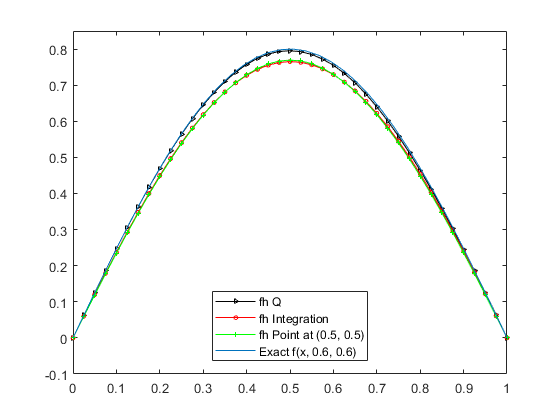
\includegraphics[width=0.75\linewidth]{../FreeFem++/fhx}\\
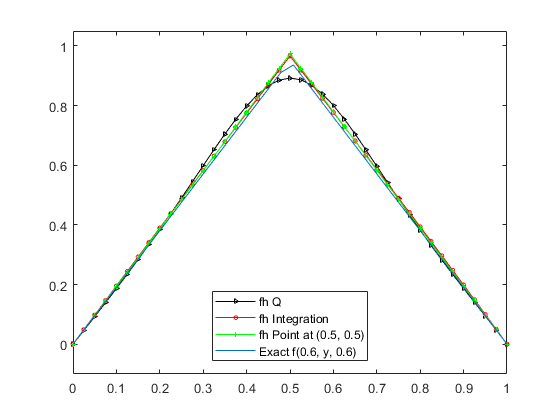
\includegraphics[width=0.75\linewidth]{../FreeFem++/fhy}\\
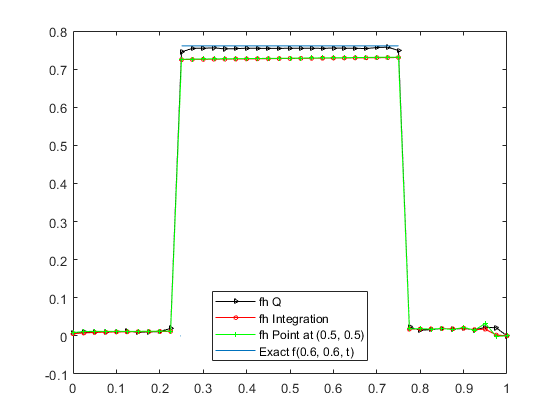
\includegraphics[width=0.75\linewidth]{../FreeFem++/fht}
\justifying
\section{Conclusion}

\bibliography{references}{}
\bibliographystyle{plain}

\end{document}
